\section{RGB}
L’extraction de RGB utilise les trois couleurs de base pour construire une image ou une vidéo : Rouge Vert et Bleu.

RGB est une paramètre de base d’une image, à l’aide de statistiques de nombre d’occurence des différentes densités de couleur dans chaque frame, la méthode p-valeur peut être mise en place pour détecter les ruptures dans une vidéo.

\subsection{Matrice RGB}

Pour ce projet, Une matrice de taille \textit{768 * NombreFrame} est construit. Les 768 lignes contiennent le nombre d'occurence des 256 densités des 3 différentes couleurs.

\subsection{Niveau de Gris}
Pour améliorer l’efficacité, le niveau de gris peut être utilisé aussi. Ce paramètre est obtenu par calculer la moyenne des trois différentes couleurs. En revanche cette solution peut déduire la précision de la détection.

\begin{figure}[h!]
      \centering
      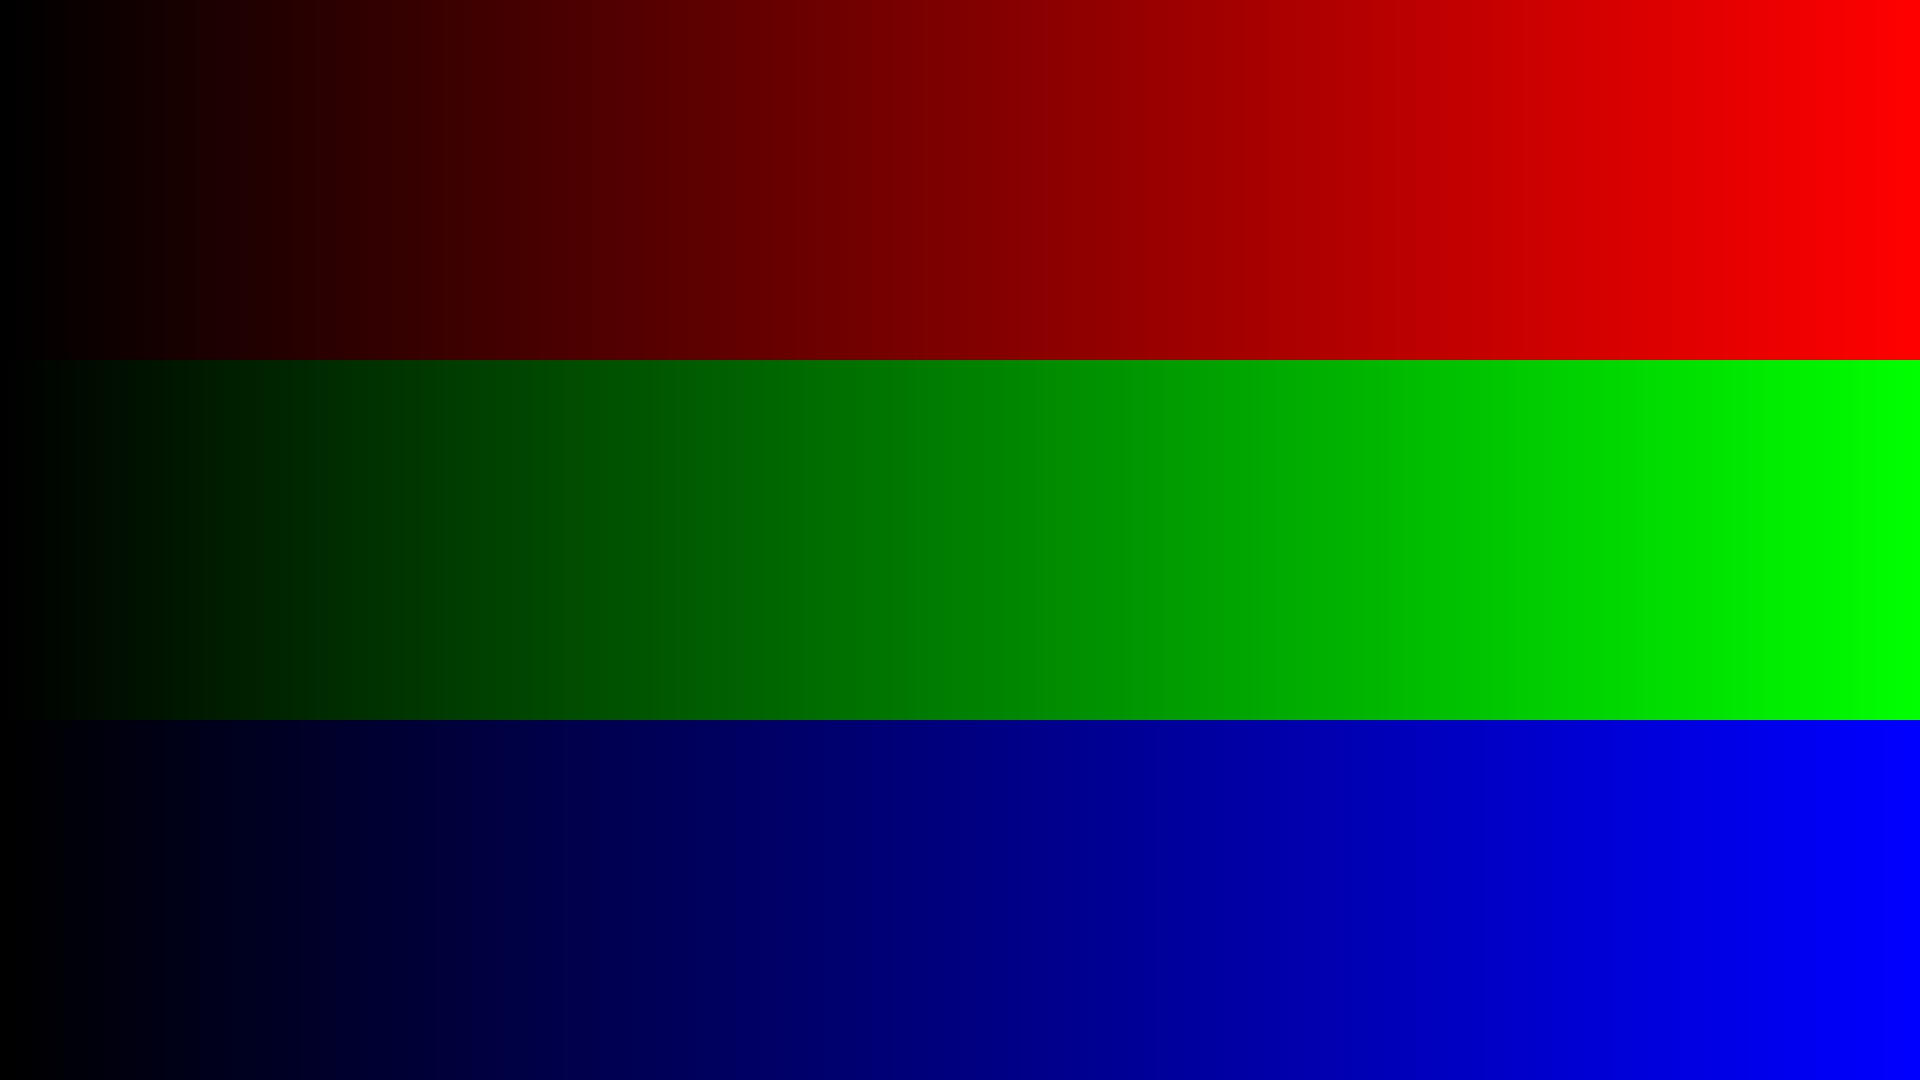
\includegraphics[scale=0.12]{images/RGB.jpg}
      \caption{\label{Après} Image après la rupture}
\end{figure}


\begin{figure}[h!]
   \begin{minipage}[c]{.46\linewidth}
	  \centering
      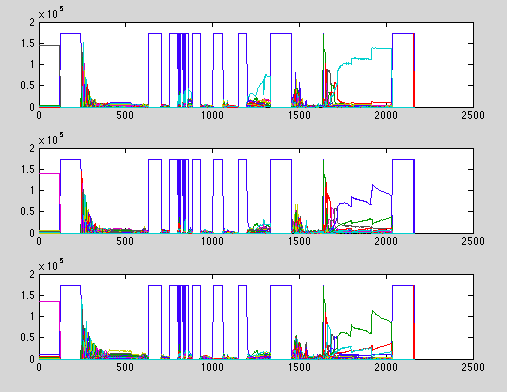
\includegraphics[scale=0.4]{images/diagRGB.png}
      \caption{\label{Avant} Image avant la rupture}
   \end{minipage} \hfill
   \begin{minipage}[c]{.46\linewidth}
      \centering
      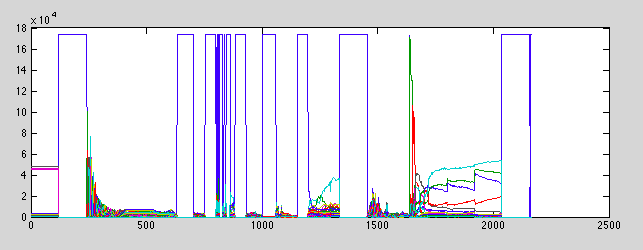
\includegraphics[scale=0.35]{images/diagGris.png}
      \caption{\label{Après} Image après la rupture}
   \end{minipage}
\end{figure}